

\chapter{Subject of the thesis}
Building Chess AI is very difficult and time consuming process if it is require to achieve good effectiveness. In scope of this thesis an approach has been used that includes the following components:
\begin{itemize}
	\item game tree as an decision making structure,
	\item min-max algorithm as a search algorithm,
	\item game tree depth limit as an optimization method,
	\item artificial neural network as a first evacuation function,
	\item convolutional neural network as a second evaluation function.
\end{itemize}

\section{Decision making system - implementation}
Starting game tree structure is generated at the beginning of the program using recursive method. At the beginning of the program, there is option to choose game tree depth limit. This configuration specify how many moves needs to be included in game tree structure. When last layer of the structure will be achieved, game tree will be destroyed and regenerated with the same depth. As it was described in section \ref{sec:game-tree-optimizations}, it is impossible to generate full game tree of chess, so that is why game tree depth limitation has been used. The most commonly used game tree depth limit is $3$. It is possible to specify different value of this parameter but it is important to keep in mind that it will impact time needed to make decision. Example structure of game tree used in the the project can be seen on \hyperref[fig:game-tree-fragment]{fig. \ref*{fig:game-tree-fragment}}.
\begin{figure}
	\centering
	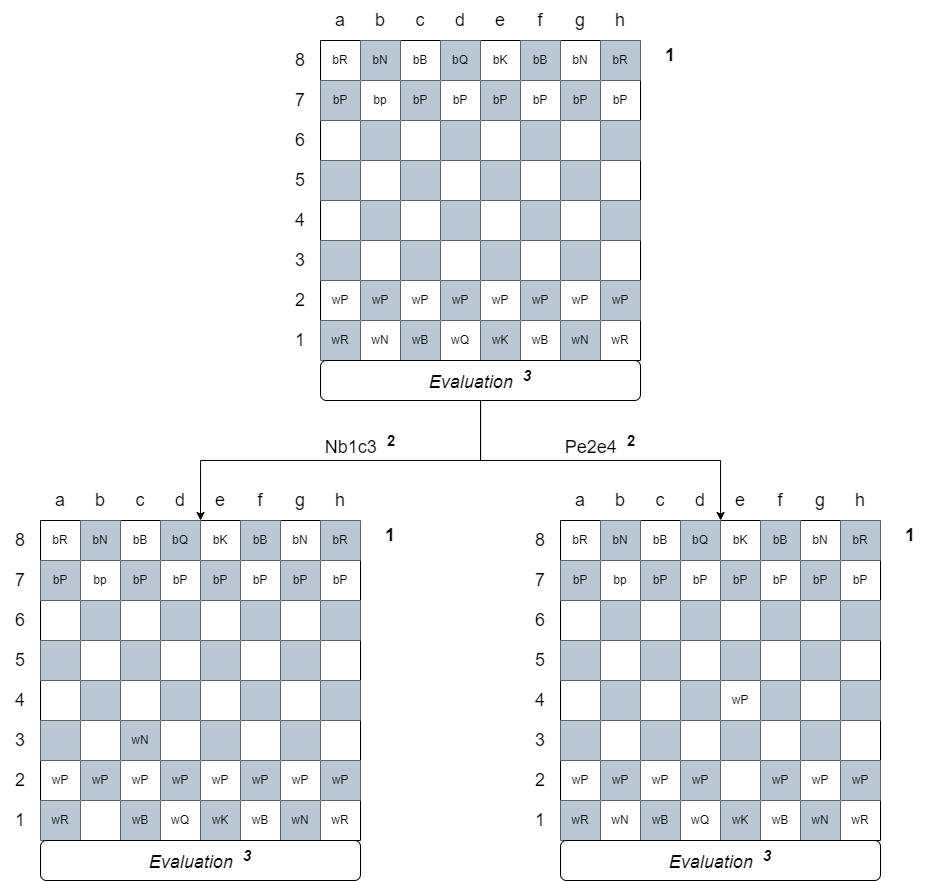
\includegraphics[width=\textwidth]{dependencies/pictures/Game_Tree_Fragment_Example.png}
	\caption{Game tree fragment example (1 - chess board representation, 2 - move command, 3 - evaluation value).}
	\label{fig:game-tree-fragment}
\end{figure}
Each game tree node, apart from the elements already mentioned, consists of list of children nodes. This list is very important component of this structure because it contains pointers to all child nodes connected to particular node. As it was mentioned in section \ref{sec:game-tree-building-process}, each chessboard situation can be connected to other situation which can be achieved by performing particular move. Process of generating list of child nodes can be described in following steps:
\begin{enumerate}
	\item Analyzing given chessboard arrangement and generate list of legal move commands for proper player
	\item For each move command generate proper chessboard arrangement
	\item Evaluate each chessboard situation and assign to it proper evaluation value
	\item Perform all previous steps for all child nodes
\end{enumerate}
This algorithm is executed until game tree depth limit is reached.

Created game tree is used as an input to the min-max search algorithm. Detail explanation of this algorithm can be found in section \ref{sec:min-max-algorithm}. There are 2 main assumptions that needs to be explain while describing usage of min-max algorithm in scope of this thesis. If game take place in scenario ,,player vs AI'', human player always is assign to white site of the board which also result in making first move. If game scenario is set to be ,,AI vs AI'', each of the instances gets assign randomly to one of the site. Sequence in which min-max algorithm work can be specified as follows:
\begin{enumerate}
	\item Find the most beneficial sequence of moves in generated game tree.
	\item Get chessboard situation after opponents move.
	\item If gathered node is not one of game tree nodes, go back to point 1. Otherwise, regenerate game tree and go back to point 1.
\end{enumerate}
Term ,,sequence of moves'', used in list above may be misleading and it needs to be further described. To avoid confusion, please note that min-max algorithm, implemented in the project, do not return list of move commands. Term ,,sequence of moves'' refers to path of nodes which was chosen by min-max algorithm. This path allows system to decide which node move command it needs to perform to achieve most beneficial situation. In conclusion, function which perform min-max algorithm, return move command that needs to be performed by AI. Important thing to mentioned is the fact that in scope of this thesis there are no optimization method used for min-max algorithm. It can result in increasing time of making decisions while playing. It was decided to use min-max tree structure because it is core element of a lot of other chess playing AI and it is the most beneficial solution. 

\section{Evaluation system - implementation}\label{sec:evaluation-system-implementation}
To make all experiments more accurate, it has been decided to implement very basic models of ANN and CNN. To increase accuracy even more, both instances were coded from scratch and trained on the same datasets. Using neural network model as an evaluation method is not a new approach but usage of CNN and ANN, on the other hand is, because the most often used models are genetic algorithm based one. It is hard to predict how effective this approach would be, before analyzing tests results, but it can be very interesting how it perform. 

Before further discursion it is necessary to describe how chessboard is represented in the final program. There are $3$ methods that chess pieces are stored: number type, string type and object type. All of those types are shown in \hyperref[tab:chess-pieces-types]{tab. \ref*{tab:chess-pieces-types}} (object type will be skipped in the table).
\begin{table}
	\centering
	\caption{The list of chess pieces types.}
	\label{tab:chess-pieces-types}
	\begin{tabular}{ccc}
	\toprule
		\textbf{symbol} & \textbf{number value} & \textbf{string value}\\
		\hline
			\WhiteKingOnWhite \BlackKingOnWhite & 7 / -7 & wK / bK\\
		\hline
			\WhiteQueenOnWhite \BlackQueenOnWhite & 5 / -5 & wQ / bQ\\
		\hline
			\WhiteBishopOnWhite \BlackBishopOnWhite & 4 / -4 & wB / bB\\
		\hline
			\WhiteKnightOnWhite \BlackKnightOnWhite & 3 / -3 & wN / bN\\
		\hline
			\WhiteRookOnWhite \BlackRookOnWhite & 2 / -2 & wR / bR\\
		\hline
			\WhitePawnOnWhite \BlackPawnOnWhite & 1 / -1 & wP / bP\\
	\end{tabular}
\end{table}
Data structure containing numerical values representing chess pieces will be used as an input in both instances of created neural networks.

\subsection{Artificial neural network - architecture}\label{sec:ann-architecture}
As it was mentioned before, each of neural network instances was implemented from scratch to make experiments more reliable. When creating artificial neural network instance, there are two main aspects that needs to be specified. First and the most crucial topic is to design architecture of the network. Because problem that needs to be solved is evaluating chessboard situation, created network needs to take $64$ values as an input (chessboard have dimension of $8 \times 8$) and needs to return one value which will be assigned as an evaluation value to the specific chessboard situation. To keep created model as simple as possible, it has been decided to include only two hidden layers with $64$ neurons each. Before further discussions about constructing neural network, it is important to mention why in both instances input data is chessboard arrangement. Because chosen approach to the given problem is to evaluate chessboard situation, it is necessary to pass arrangement of all pieces on the board to the neural network. Before passing chessboard representation into ANN it is necessary to reshape input data to be vector of size $64$. data prepared this way can be mapped into proper input layer neurons. Process of specifying neural network structure is very hard because there are not that many regulations or patterns that can be followed. One of the patterns that can make this process easier is to decide what task will be perform by which hidden layer. Unfortunately it is impossible to predict if layers in final model will really perform assumed tasks but making this kind of assumptions is very helpful while designing ANN structure. It has been decided that first hidden layer will be responsible for specifying each chessboard field profit value. Second hidden layer on the other hand will be responsible for calculating each chessboard field profit value based on the values calculated in previous layer. While analyzing this topic, there were an idea to add one additional hidden layer with $4$ neurons, which will be responsible for specifying impact of following situations on final evaluation: 
\begin{itemize}
	\item final value of pieces on chessboard (sum of all pieces left on the chessboard),
	\item check status,
	\item checkmate status.
\end{itemize}
However, it was decided that this hidden layer would not be implemented in the final structure of the network. Last thing that need to be described related to network architecture is output layer. As it was mentioned in section \ref{sec:ann-architecture} output layer is treated as an network answer for given problem. In case of this thesis created ANN will return only one value which represent how beneficial for particular player is given chessboard situation. The smallest returned value, less beneficial given situation is for respective player. Even if it is ver unlikely, it is possible that network will return value $0$. This mean that particular situation is neutral for both players. When structure of the network has been created, there is one last important configuration to establish. As it was mentioned in section \ref{sec:learning-process-for-nn-instance}, every instance of neural network needs to have learning rate parameter specified. During training process, it was established that learning rate value for artificial neural network should be equal to $0.001$. This value resulted in the most efficient training process for this model. It is possible that ANN evaluation function will not provide spectacular results for given problem but it is important to remember that it has been used as an basic point of comparison for second evaluation. This method allows to decide if usage of CNN, for evaluating chessboard situations, is an justified or beneficial solution to the problem.

Last thing worth describing in this section is method of creating ANN instance in final project. Because every component of the network has been implemented from scratch, creation process also needed to be implemented. Artificial neural network is created base on \textbf{topology}. It is list of numbers which define structure of the model. This solution can be implemented for this type of network because it use only one type of layer which is fully connected layer. There are two requirements which topology structure have to meet:
\begin{itemize}
	\item list cannot be smaller than $2$,
	\item values in the list must be grater than $0$.
\end{itemize}
Each value in topology object specify number of neurons in respective layer. Using those information, all necessary layers are created with respective sizes, specified in topology.

\subsection{Convolutional neural network - architecture}\label{sec:cnn-architecture}
While planing structure for convolutional neural network, the main goal was to keep structure of the model simple. This decision has been made because if basic structure of CNN model won't perform better than basic structure of ANN, it is a proof that given solution is bad. Second reason for keeping model structure simple is less time consuming training process for both models. There are two elements in convolutional neural network configuration that are similar to the first used model. The best value for learning rate parameter is equal to $0.001$ and sizes of input and output layers are also the same like in artificial neural network. Function and meaning of input and output layers are the same in both used types of networks. It has been decided that CNN model will consists of two convolutional layers, with $13$ and $10$ kernels respectively, two pooling layers, two activation layers and one fully connected layer. Full structure of the used CNN can be found on \hyperref[fig:cnn-structure]{fig. \ref*{fig:cnn-structure}}.
\begin{figure}
	\centering
	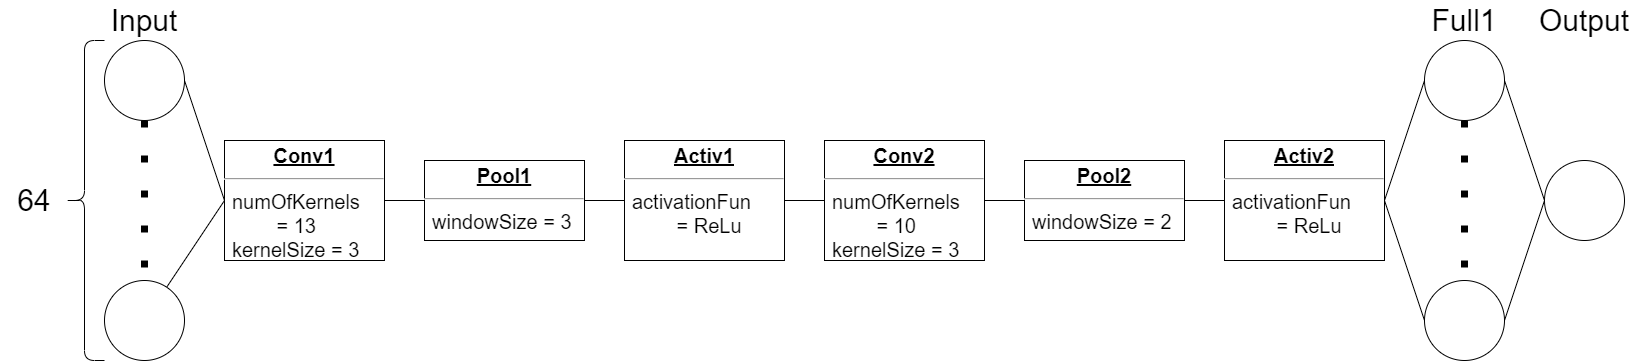
\includegraphics[width=\textwidth]{dependencies/pictures/CNN_Structure.png}
	\caption{Structure of the implemented CNN (Conv - convolutional layer, Pool - pooling layer, Activ - activation layer, Full - fully connected layer).}
	\label{fig:cnn-structure}
\end{figure}
In the contrary to ANN hidden layers, which number of neurons are not backed by any theoretical aspects, convolutional layers was design based on chess game theory. According to publications about chess there are $13$ best openings which give player the most benefits. This information helped establish the most optimal number of kernels in first convolutional layer (\textbf{Conv1} on \hyperref[fig:cnn-structure]{fig. \ref*{fig:cnn-structure}}). By specifying $13$ kernels in the first layer, it is assumed that it will be able to recognize beneficial opening patterns on the chessboard. Second information that chess publication provided was general beneficial chessboard arrangements that could happened in the course of the game. There are $10$ of those arrangements \cite{bib:book-mastering-chess-logic,bib:book-chess-bible,bib:book-bobby-fisher-teaches-chess} and that is why second convolutional layer (\textbf{Conv2} on \hyperref[fig:cnn-structure]{fig. \ref*{fig:cnn-structure}}) consists of this number of kernels. Similarly like in first convolutional layer, this one is also assumed to be able to recognize patterns mentioned in used publications. Last thing worth mentioning about used convolutional layers is size of the kernel. Both of the layers uses the same kernel size of $3$. This parameter has been initialize with this value because according to used publications, in range $3 \times 3$ around chess piece it is possible to detect the biggest number of patterns and potential dangers \cite{bib:book-mastering-chess-logic,bib:book-chess-bible,bib:book-bobby-fisher-teaches-chess}. 

Next, used type of layer is pooling layer. As it was described in section \ref{sec:cnn-architecture}, it is used to reduce size of the matrices for further calculations. First pooling layer (\textbf{Pool1} on \hyperref[fig:cnn-structure]{fig. \ref*{fig:cnn-structure}}) consists of pooling window of size $3$. This window is bigger than the one used in second poling layer (\textbf{Pool2} on \hyperref[fig:cnn-structure]{fig. \ref*{fig:cnn-structure}}) and because of it, it will make output matrices 3 times smaller. Matrices gathered from first convolutional layer can be smaller because as it was mentioned before those feature maps represent opening situations. According to used chess publications, opening situations happens in smaller chessboard scope (three first rows of the chessboard) which allows for bigger reduction in features maps sizes. For second pooling layer, pooling window of size $2$ has been used. It was configure this way because general beneficial situation can happened in full scope of the chessboard which greatly reduces the possibility of reducing the output matrices sizes. If these matrices were too small, this could lead to some important information being omitted from further processing.

Last two types of layer, used in CNN architecture do not need that much description. Both of activation layers, use \textbf{ReLu} activation function to change values in matrices into activation values. It has been decided to use ReLu function because according to used publications about convolutional neural networks, this activation function is the most commonly used while creating this type fo networks \cite{bib:book-statistical-learning,bib:book-generative-deep-learning}. Fully connected layer, at the end of the network has been used to provide output of the correct dimension for output layer. Because output layer is also fully connected layer it is impossible to calculate output evaluation using list of matrices generated by previous layers. Gathered matrices needs to be converted into fully connected layer which will later be used for calculating network answer.

Creation process, for this type of network, has been implemented differentially than in case of ANN model. It is because CNN can consists of more than one type of layer. Because each of layer types needs different initialization parameters, construction process has been implemented based on adding new layers manually. To end creation process, output layer needs to be added. Output layer can be added to the model by calling special function.

\subsection{Training system - implementation}
Training of both neural network instances has been performed in separation of application core. Separate project has been created and all necessary modules has been loaded into it. Using this project, training process has been performed. Full training looks as follows:
\begin{description}
	\item[Load training data] -- read training data and save it in data set object.
	\item[Split data set] -- divide created data set object into train set and test set.
	\item[Shuffle data set] -- shuffle examples in train set (it is important to remember that shuffling can be performed only for training set) 
	\item[Train] -- process all examples in train set and update weights and biases.
	\item[Validate] -- process all examples from test set and gather results.
	\item[Calculate accuracy] -- check how accurate each answers were and calculate full accuracy of the model.
	\item[Contunue] -- if accuracy is acceptable end training, if it is not acceptable go back to step ,,train''.
	\item[Save model] -- save parameters values of given model into JSON file.  
\end{description}
It is important to mention that training process looks the same for both neural networks. For both networks training, the same dataset is used. After training process finish, it is possible to save neural network configuration in JSON file. This feature has been implemented to allows loading already trained models. Example of file with saved network configuration can be see on \hyperref[fig:saved-weights-example-ann]{fig. \ref*{fig:saved-weights-example-ann}}.
\begin{figure}
	\centering
	\begin{lstlisting}
		"name": "NN 1",
		"layer1": {
			"inputWeights": [
				0.1,
				0.4
			]
		},
		"bias1": 0.2,
		"layer2": {
			"inputWeights": [
				0.5
			]
		},
		"bias2": 0.3
	\end{lstlisting}
	\caption{Example of file containing saved ANN model configuration.}
	\label{fig:saved-weights-example-ann}
\end{figure}
Before describing construction of mentioned file, it is important to notice that the used example shows very basic neural network configuration. \hyperref[fig:saved-weights-example-ann]{Figure \ref*{fig:saved-weights-example-ann}} do not present configuration of neural network instance used to resolve given problem. This decision has been made because both instances of neural network, used in final project, would take to much place in final JSON file for it to be readable. One last remark, given example present saved configuration of ANN type of network but configuration for CNN looks similar. Example of file containing configuration of CNN is presented on \hyperref[fig:saved-weights-example-cnn]{fig. \ref*{fig:saved-weights-example-cnn}}.
\begin{figure}
	\centering
	\begin{lstlisting}
		"name": "NN 2",
		"layer1": {
			"inputWeights": [
				[ 0.1, 0.5 ],
				[ 0.4, 0.9 ]
			]
		},
		"bias1": [
			[ 0.3, 0.3 ],
			[ 0.6, 0.1 ]
		],
		"layer2": {
			"inputWeights": [
				[ 0.7 ]
			]
		},
		"bias2": [
			[ 0.5, 0.2 ],
			[ 0.9, 0.2 ]
		]
	\end{lstlisting}
	\caption{Example of file containing saved CNN model configuration.}
	\label{fig:saved-weights-example-cnn}
\end{figure}
As it can be seen, only difference between ANN and CNN configuration is the fact that for CNN, layer weights are represented by matrices. Information that gets saved inside configuration file are: network name, definition of each configurable layer and biases. All of data that can be found in configuration file are configurable parameter of particular type of neural network. By saving those information, trained model can be loaded for further use.

\section{Used tools}
In the scope this thesis, all components of the final project has been implemented from scratch using C++17 language. As an IDE Visual Studio Code (VSCode) has been chosen. To build and prepare project for compilation Premake software has been used. This thesis has been written using \LaTeX language and VSCode IDE. For creating all diagrams used in this thesis, Draw.io online software has been used. In the creative process of this project, the sources included in the bibliography and following documentations were used: \cite{bib:internet-c++-doc,bib:internet-latex-doc,bib:internet-vscode-doc,bib:internet-premake-doc}.

% tekst

% \section{[Section title]}

% \section{[Subsection title]}

% Each figure in the document should be referred to at least once (fig. \ref{fig:2}).

% \begin{figure}
% \centering
% \begin{tikzpicture}
% \begin{axis}[
%     y tick label style={
%         /pgf/number format/.cd,
%             fixed,   % po zakomentowaniu os rzednych jest indeksowana wykladniczo
%             fixed zerofill, % 1.0 zamiast 1
%             precision=1,
%         /tikz/.cd
%     },
%     x tick label style={
%         /pgf/number format/.cd,
%             fixed,
%             fixed zerofill,
%             precision=2,
%         /tikz/.cd
%     }
% ]
% \addplot [domain=0.0:0.1] {rnd};
% \end{axis} 
% \end{tikzpicture}
% \caption{Figure caption.} % Figure caption is BELOW the figure!
% \label{fig:2}
% \end{figure}

% Each table in the document should be referred to at least once (Tab. \ref{tab:results}).

% \begin{table}
% \centering
% \caption{A caption of a table is ABOVE it.}
% \label{tab:results}
% \begin{tabular}{rrrrrrrr}
% \toprule
% 	         &                                     \multicolumn{7}{c}{method}                                      \\
% 	         \cmidrule{2-8}
% 	         &         &         &        \multicolumn{3}{c}{alg. 3}        & \multicolumn{2}{c}{alg. 4, $\gamma = 2$} \\
% 	         \cmidrule(r){4-6}\cmidrule(r){7-8}
% 	$\zeta$ &     alg. 1 &   alg. 2 & $\alpha= 1.5$ & $\alpha= 2$ & $\alpha= 3$ &   $\beta = 0.1$  &   $\beta = -0.1$ \\
% \midrule
% 	       0 &  8.3250 & 1.45305 &       7.5791 &    14.8517 &    20.0028 & 1.16396 &                       1.1365 \\
% 	       5 &  0.6111 & 2.27126 &       6.9952 &    13.8560 &    18.6064 & 1.18659 &                       1.1630 \\
% 	      10 & 11.6126 & 2.69218 &       6.2520 &    12.5202 &    16.8278 & 1.23180 &                       1.2045 \\
% 	      15 &  0.5665 & 2.95046 &       5.7753 &    11.4588 &    15.4837 & 1.25131 &                       1.2614 \\
% 	      20 & 15.8728 & 3.07225 &       5.3071 &    10.3935 &    13.8738 & 1.25307 &                       1.2217 \\
% 	      25 &  0.9791 & 3.19034 &       5.4575 &     9.9533 &    13.0721 & 1.27104 &                       1.2640 \\
% 	      30 &  2.0228 & 3.27474 &       5.7461 &     9.7164 &    12.2637 & 1.33404 &                       1.3209 \\
% 	      35 & 13.4210 & 3.36086 &       6.6735 &    10.0442 &    12.0270 & 1.35385 &                       1.3059 \\
% 	      40 & 13.2226 & 3.36420 &       7.7248 &    10.4495 &    12.0379 & 1.34919 &                       1.2768 \\
% 	      45 & 12.8445 & 3.47436 &       8.5539 &    10.8552 &    12.2773 & 1.42303 &                       1.4362 \\
% 	      50 & 12.9245 & 3.58228 &       9.2702 &    11.2183 &    12.3990 & 1.40922 &                       1.3724 \\
% \bottomrule
% \end{tabular}
% \end{table}  


%\chapter{[Subject of the thesis]}
%
%\begin{itemize}
%\item solution to the problem proposed by the author of the thesis
%\item theoretical analysis of proposed solutions
%\item rationale of applied methods, algorithms, and tools
%\end{itemize}